\documentclass[12pt,a4paper]{report}

% ─── Packages ────────────────────────────────────────────────────────────────
\usepackage[T1]{fontenc}
\usepackage[utf8]{inputenc}

\usepackage[a4paper, margin=2.5cm]{geometry}
\usepackage{graphicx}
\usepackage{booktabs}
\usepackage{longtable}
\usepackage{array}
\usepackage{tabularx}
\usepackage{xcolor}
\usepackage{listings}
\usepackage{hyperref}
\usepackage{fancyhdr}
\usepackage{titlesec}
\usepackage{setspace}
\usepackage{caption}
\usepackage{subcaption}
\usepackage{amsmath}
\usepackage{float}
\usepackage{parskip}
\usepackage{enumitem}

\usepackage{pdfpages}

% ─── Colours ─────────────────────────────────────────────────────────────────
\definecolor{codebg}{RGB}{248,248,248}
\definecolor{codeframe}{RGB}{200,200,200}
\definecolor{keywordcolor}{RGB}{0,0,180}
\definecolor{commentcolor}{RGB}{60,120,60}
\definecolor{stringcolor}{RGB}{160,0,0}
\definecolor{headingblue}{RGB}{31,73,125}

% ─── Hyperref ─────────────────────────────────────────────────────────────────
\hypersetup{
    colorlinks=true,
    linkcolor=headingblue,
    urlcolor=headingblue,
    citecolor=headingblue,
    pdftitle={Design and Implementation of an SPI Communication Interface on FPGA},
    pdfauthor={Molik Rajvanshi, Shivam Tiwari, Ujjawal Khatri},
}

% ─── Listings (code) ──────────────────────────────────────────────────────────
\lstdefinelanguage{Verilog}{
    keywords={module, endmodule, input, output, reg, wire, parameter, localparam,
              always, if, else, begin, end, case, endcase, default, assign,
              posedge, negedge, initial, task, endtask, repeat, for, integer},
    keywordstyle=\color{keywordcolor}\bfseries,
    comment=[l]{//},
    commentstyle=\color{commentcolor}\itshape,
    morecomment=[s]{/*}{*/},
    stringstyle=\color{stringcolor},
    sensitive=true,
}

\lstdefinelanguage{XDC}{
    keywords={set\_property, create\_clock, get\_ports},
    keywordstyle=\color{keywordcolor}\bfseries,
    comment=[l]{\#\#},
    commentstyle=\color{commentcolor}\itshape,
    sensitive=false,
}

\lstdefinelanguage{Arduino}{
    keywords={void, int, uint8_t, bool, volatile, if, else, while, for,
              return, ISR, noInterrupts, interrupts, Serial, pinMode,
              INPUT, OUTPUT, HIGH, LOW, true, false, sei},
    keywordstyle=\color{keywordcolor}\bfseries,
    comment=[l]{//},
    commentstyle=\color{commentcolor}\itshape,
    morecomment=[s]{/*}{*/},
    stringstyle=\color{stringcolor},
    sensitive=true,
}

\lstset{
    backgroundcolor=\color{codebg},
    frame=single,
    rulecolor=\color{codeframe},
    basicstyle=\ttfamily\footnotesize,
    breaklines=true,
    breakatwhitespace=false,
    keepspaces=true,
    showspaces=false,
    showstringspaces=false,
    tabsize=4,
    captionpos=b,
    numbers=left,
    numberstyle=\tiny\color{gray},
    numbersep=8pt,
    xleftmargin=15pt,
    xrightmargin=5pt,
}

% ─── Section heading styles ───────────────────────────────────────────────────
\titleformat{\chapter}[block]
  {\normalfont\Large\bfseries\color{headingblue}}
  {\thechapter.}{0.5em}{}
\titlespacing*{\chapter}{0pt}{10pt}{15pt}

\titleformat{\section}
  {\normalfont\large\bfseries\color{headingblue}}
  {\thesection}{0.5em}{}

\titleformat{\subsection}
  {\normalfont\normalsize\bfseries\color{headingblue}}
  {\thesubsection}{0.5em}{}

% ─── Header / Footer ─────────────────────────────────────────────────────────
\pagestyle{fancy}
\fancyhf{}
\fancyhead[L]{\small SPI Communication Interface on FPGA}
\fancyhead[R]{\small B.Tech ECE Project}
\fancyfoot[C]{\thepage}
\renewcommand{\headrulewidth}{0.4pt}

% ─── Misc helpers ────────────────────────────────────────────────────────────
\setlength{\parskip}{6pt}
\setlength{\parindent}{0pt}
\captionsetup{font=small, labelfont=bf}

% ─────────────────────────────────────────────────────────────────────────────
\begin{document}

% ══════════════════════════════════════════════════════════════════════════════
%  TITLE PAGE
% ══════════════════════════════════════════════════════════════════════════════
\begin{titlepage}
  \centering
  \vspace*{1.5cm}

  % ── Title ──────────────────────────────────────────────────────────────────
  {\LARGE\bfseries
    Design and Implementation of an SPI Communication\\[6pt]
    Interface on FPGA\par}

  \vspace{1.2cm}

  % ── Submission statement ───────────────────────────────────────────────────
  {\normalsize Project submitted for the fulfillment of the\par}
  \vspace{0.3cm}
  {\normalsize Requirements of the degree of\par}

  \vspace{0.8cm}

  {\normalsize Bachelor of Technology\par}
  \vspace{0.2cm}
  {\normalsize Electronics and Communication Technology\par}

  \vspace{1.2cm}

  % ── Authors ────────────────────────────────────────────────────────────────
  {\normalsize
    Molik Rajvanshi- 23UEC575\\[3pt]
    Shivam Tiwari- 23UEC622\\[3pt]
    Ujjawal Khatri- 23UEC635\par}

  \vspace{0.5cm}

  {\normalsize
    Email :
    \href{mailto:23uec575@lnmiit.ac.in}{23uec575@lnmiit.ac.in}\\[2pt]
    \phantom{Email :\ }
    \href{mailto:23uec622@lnmiit.ac.in}{23uec622@lnmiit.ac.in}\\[2pt]
    \phantom{Email :\ }
    \href{mailto:23uec635@lnmiit.ac.in}{23uec635@lnmiit.ac.in}\par}

  \vspace{1.2cm}

  % ── Supervisor ─────────────────────────────────────────────────────────────
  {\normalsize
    Project Supervisor-:\\[3pt]
    Dr. Kusum Lata\par}

  \vspace{1.0cm}

  % ── Logo ───────────────────────────────────────────────────────────────────
  
\includegraphics[width=5cm]{images/lnmiit_logo.png}

  \vspace{0.75cm}

  % ── Department ─────────────────────────────────────────────────────────────
  {\normalsize
    Department of Electronics and Communication\\
    Engineering- The LNM Institute of Information\\
    Technology, Jaipur\par}

\end{titlepage}

% ══════════════════════════════════════════════════════════════════════════════
%  TABLE OF CONTENTS
% ══════════════════════════════════════════════════════════════════════════════
\tableofcontents
\listoffigures
\listoftables
\newpage

% ══════════════════════════════════════════════════════════════════════════════
\chapter{Objective}
% ══════════════════════════════════════════════════════════════════════════════

This project designs and implements a complete Serial Peripheral Interface (SPI) communication system between an Artix-7 FPGA (Nexys 4 DDR) and an Arduino Uno microcontroller. The FPGA acts as the SPI master and the Arduino as the hardware SPI slave.

The user sets an 8-bit value on SW[7:0] and presses BTND. The FPGA transmits that byte over the SPI bus. The Arduino receives it, prints the value on the Serial Monitor, increments it by one, and returns the result. The FPGA then displays the received (SW+1) value on LED[7:0], while LED[15] illuminates during the transfer.

\textbf{Specific objectives:}
\begin{itemize}[leftmargin=1.5em]
  \item Implement a fully synchronous SPI Mode 0 (CPOL=0, CPHA=0) master FSM in Verilog on the Nexys 4 DDR.
  \item Design a 2-stage synchronizer and stable-counter debouncer for the send button (BTND).
  \item Interface with an Arduino Uno as an ISR-driven hardware SPI slave.
  \item Demonstrate full-duplex 8-bit data transfer at 1\,MHz SPI clock over Pmod JA.
  \item Protect the FPGA I/O from 5\,V Arduino MISO using a passive voltage divider.
  \item Verify correct operation with at least 5 hardware observations and a simulation testbench.
\end{itemize}

% ══════════════════════════════════════════════════════════════════════════════
\chapter{Tools and Resources Used}
% ══════════════════════════════════════════════════════════════════════════════

\begin{itemize}[leftmargin=1.5em]
  \item \textbf{Development Board:} Nexys 4 DDR --- Xilinx Artix-7 XC7A100T-1CSG324C, 100\,MHz on-board oscillator.
  \item \textbf{Design Software:} Vivado 2022.1 --- for synthesis, implementation, bitstream generation, and behavioral simulation.
  \item \textbf{Languages Used:} Verilog (FPGA modules and testbench), C++ (Arduino sketch using AVR SPI registers).
  \item \textbf{Additional Tools:} Arduino IDE 2.x --- for compiling and uploading the SPI slave sketch; Serial Monitor at 115200 baud.
  \item \textbf{IP Cores Used:} None --- all logic (FSM, clock divider, debouncer) implemented manually for learning purposes.
  \item \textbf{Passive Components:} 1\,k$\Omega$ and 2\,k$\Omega$ resistors (voltage divider on MISO line), breadboard, jumper wires.
\end{itemize}

% ══════════════════════════════════════════════════════════════════════════════
\chapter{System Design / Architecture}
% ══════════════════════════════════════════════════════════════════════════════

\section{System Block Diagram}

The system connects a Nexys 4 DDR FPGA (acting as SPI master) to an Arduino Uno (acting as SPI slave). The user controls the transmitted data via DIP switches (SW[7:0]) and triggers each transfer with a button press (BTND). The received response is displayed on the LED array.

\begin{figure}[H]
  \centering
  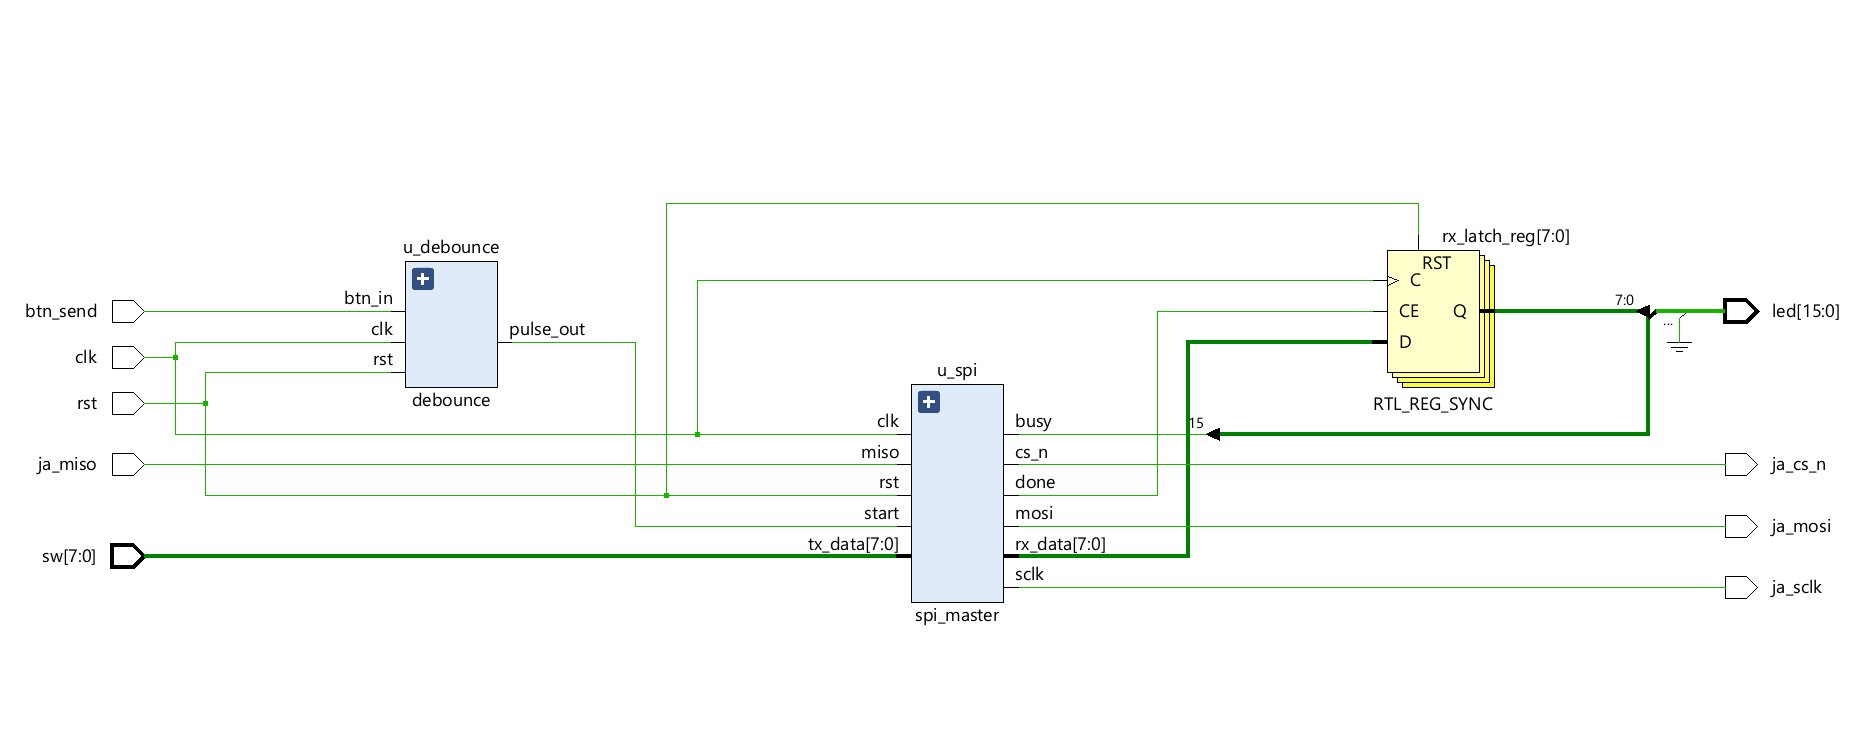
\includegraphics[width=0.95\linewidth]{images/rtl_schematic.png}
  \caption{Vivado-generated RTL schematic showing module hierarchy and signal routing (system architecture: data flow from switches to FPGA SPI master to Arduino and back to LEDs)}
  \label{fig:block_diagram}
\end{figure}

\section{Module Descriptions}

The design consists of three synthesizable Verilog modules and one constraints file:

\textbf{\texttt{spi\_master.v}} \\
The core of the design. Implements a 3-state Mealy/Moore FSM (IDLE, TRANSFER, FINISH) driving all four SPI signals. A 3-bit bit counter tracks progress through the 8-bit frame. A half-period counter (\texttt{clk\_cnt}) divides the 100\,MHz system clock by $2 \times \text{CLK\_DIV} = 100$, producing a 1\,MHz SPI clock. MOSI is driven on the falling SCLK edge; MISO is sampled on the rising edge --- complying with Mode 0 timing. The \texttt{done} output pulses for exactly one system clock cycle when the transaction is complete and \texttt{rx\_data} is valid.

\textbf{\texttt{debounce.v}} \\
A 2-stage synchronizer removes metastability from the asynchronous button input. A 20-bit stable counter counts 1\,000\,000 consecutive stable cycles (10\,ms at 100\,MHz) before accepting a level change. A rising-edge detector generates a single-cycle \texttt{pulse\_out}, ensuring \texttt{spi\_master.start} is asserted for exactly one clock cycle per button press regardless of how long the user holds the button.

\textbf{\texttt{top.v}} \\
The top-level wrapper instantiates \texttt{debounce} and \texttt{spi\_master}, connects them, and latches \texttt{rx\_data} into an 8-bit register on the rising edge of \texttt{done}. This hold register ensures LED[7:0] retains the received value between transfers rather than going dark. LED[15] is wired directly to the \texttt{spi\_master busy} flag for real-time visual feedback.

\section{SPI FSM Diagram}

\begin{figure}[H]
  \centering
  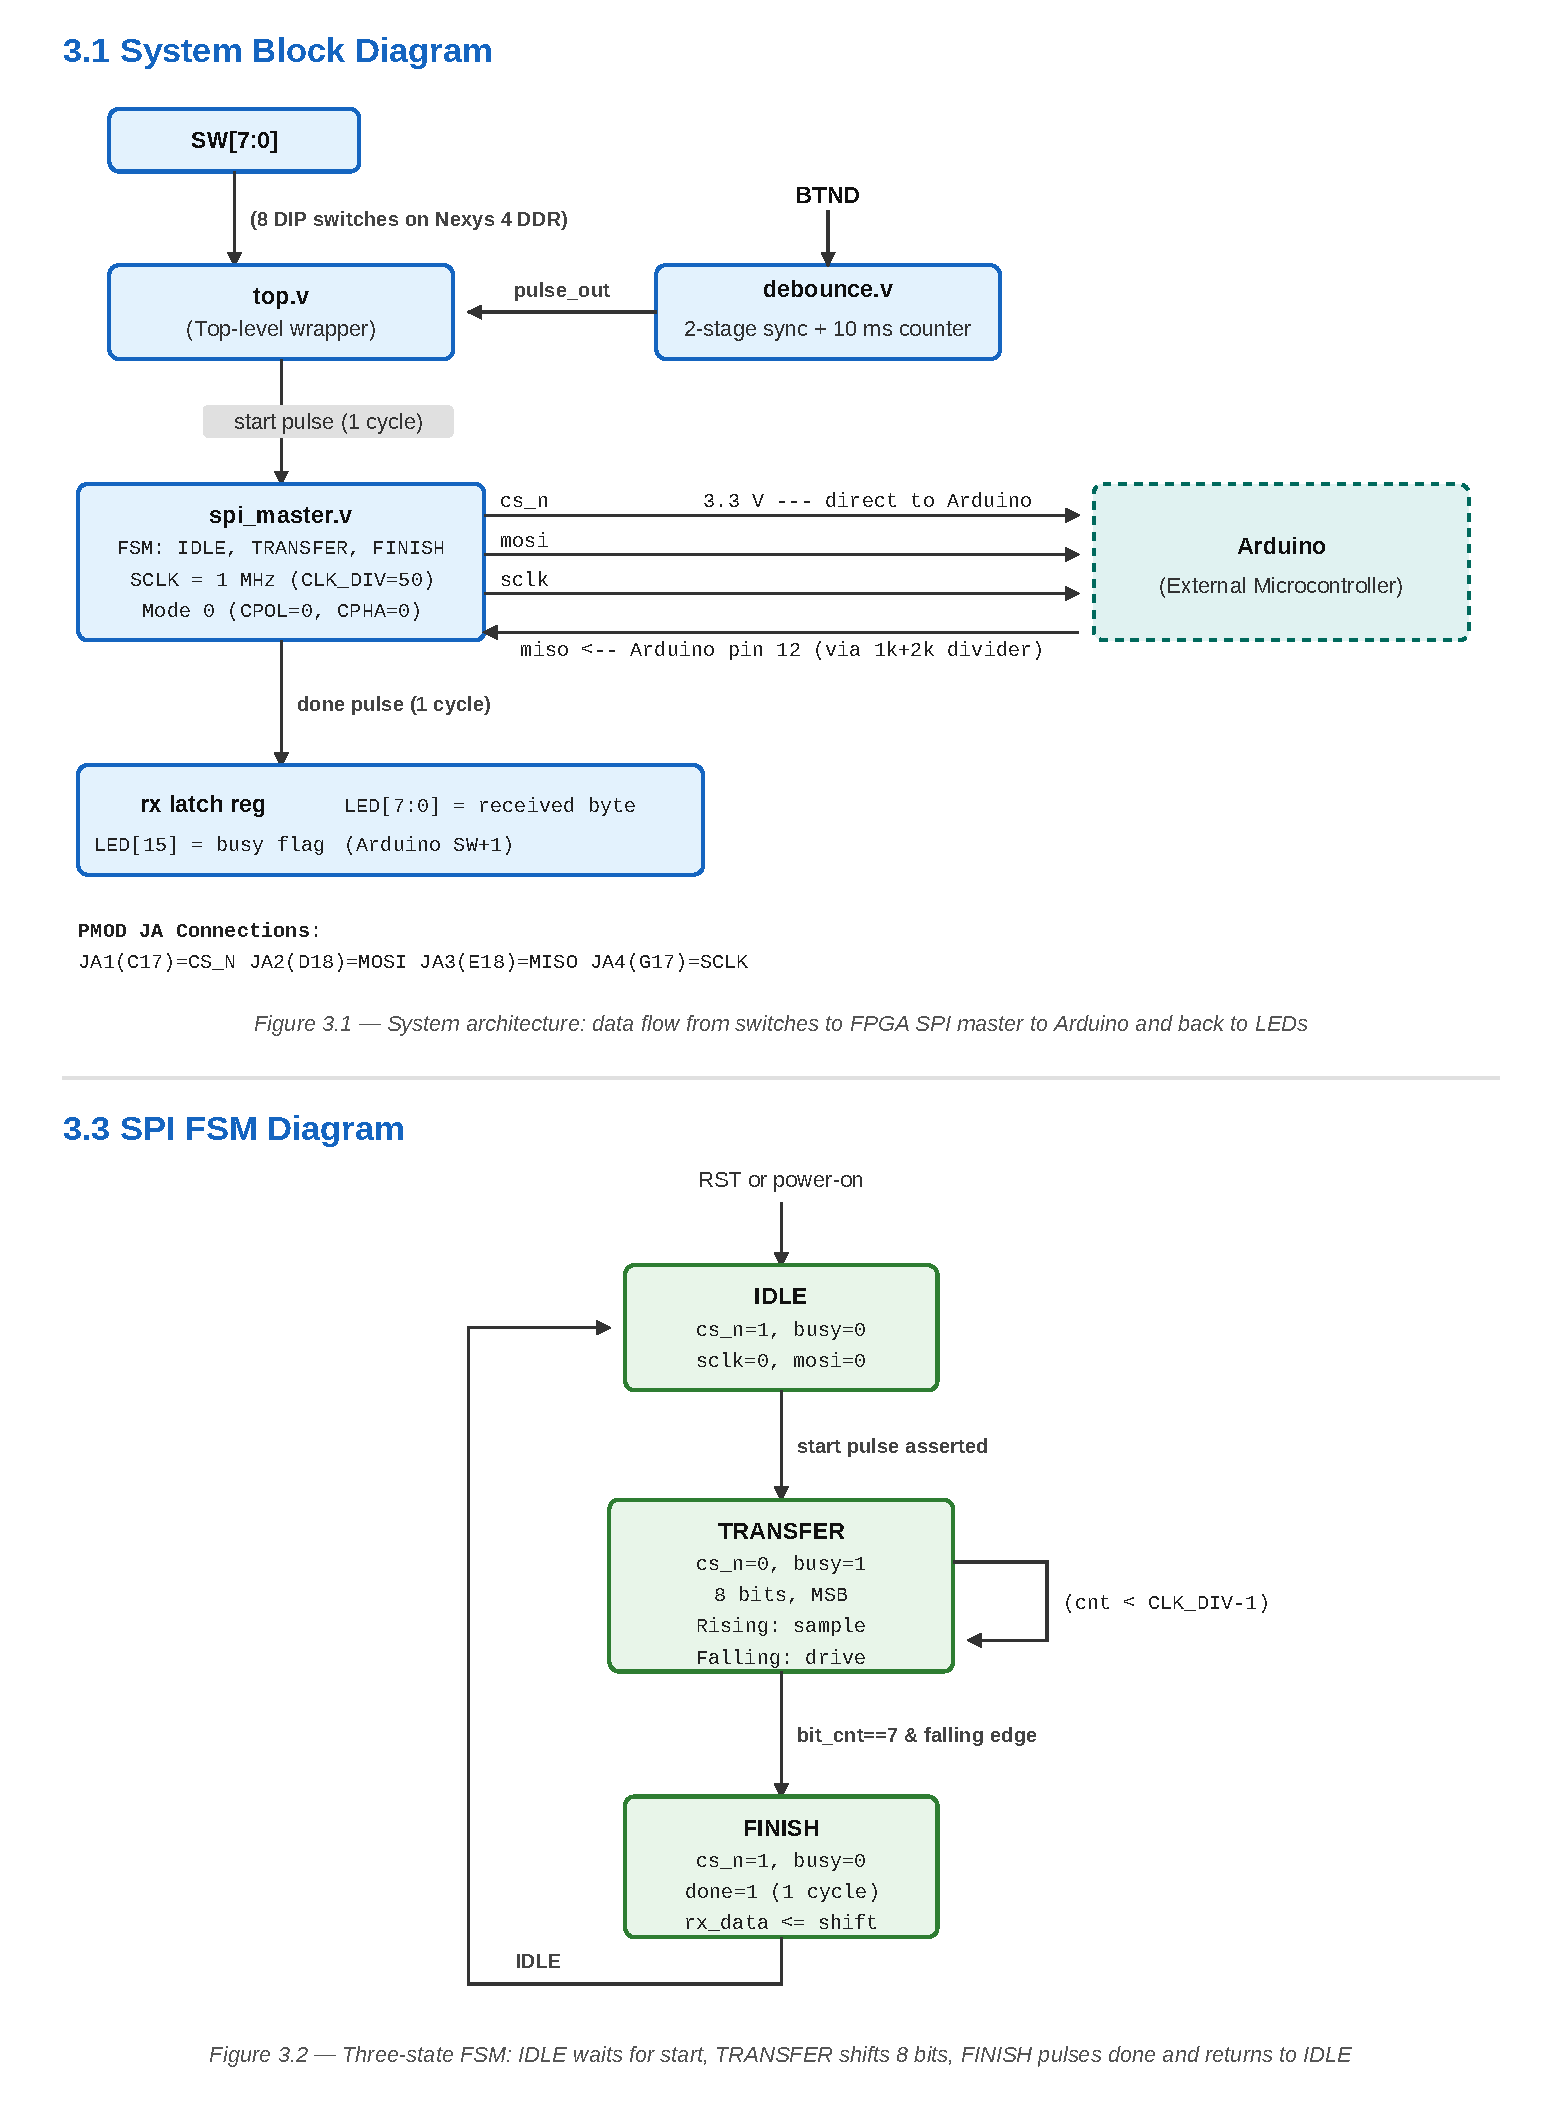
\includegraphics[width=0.80\linewidth]{images/fsm_diagram.pdf}
  \caption{Three-state FSM: IDLE waits for start, TRANSFER shifts 8 bits, FINISH pulses done and returns to IDLE}
  \label{fig:fsm}
\end{figure}

\section{SPI Mode 0 Timing Diagram}

SPI Mode 0 (CPOL=0, CPHA=0) timing is defined as follows:
\begin{itemize}[leftmargin=1.5em]
  \item MOSI is driven on the \textbf{falling} SCLK edge.
  \item MISO is sampled on the \textbf{rising} SCLK edge.
  \item CS\_N is asserted (LOW) for the full duration of the 8-bit frame, with a one-clock idle period before and after.
\end{itemize}

\vspace{4pt}
\textbf{Legend:} \texttt{X} = asserted for exactly 1 clock cycle. CS\_N brackets the entire SPI frame.

\section{Voltage Level Protection}

The FPGA Pmod pins are strictly 3.3\,V (LVCMOS33). Arduino Uno MISO is 5\,V. A resistive divider (Arduino pin 12 $\to$ 1\,k$\Omega$ $\to$ junction $\to$ 2\,k$\Omega$ $\to$ GND) produces
\[
  V_\text{junction} = 5 \times \frac{2}{3} \approx 3.33\,\text{V}
\]
at the junction, which connects to FPGA JA pin 3. The FPGA output signals (MOSI, SCLK, CS\_N) at 3.3\,V are recognised as logic HIGH by the Arduino ($V_{IH} = 2.0\,\text{V}$), so no level shifting is needed for those lines.

% ══════════════════════════════════════════════════════════════════════════════
\chapter{Implementation}
% ══════════════════════════════════════════════════════════════════════════════

\section{Vivado Project Steps}

\begin{enumerate}[leftmargin=1.5em]
  \item Create a new RTL project in Vivado 2022.1; target device: \texttt{xc7a100tcsg324-1}.
  \item Add \texttt{logic.v} (spi\_master), \texttt{debounce.v}, and \texttt{top.v} as design sources. Set \texttt{top} as top module.
  \item Add \texttt{nexys4ddr.xdc} as a constraints source.
  \item Run Synthesis $\to$ Implementation $\to$ Generate Bitstream.
  \item Open Hardware Manager, connect Nexys 4 DDR via USB-JTAG, and program the device.
\end{enumerate}

\section{Arduino Setup}

\begin{enumerate}[leftmargin=1.5em]
  \item Open \texttt{arduino\_spi\_slave.ino} in Arduino IDE 2.x.
  \item Select Board: Arduino Uno, correct COM port.
  \item Upload the sketch.
  \item Open Serial Monitor at 115200 baud before triggering the FPGA.
\end{enumerate}

\section{Pin Assignments}

\begin{table}[H]
  \centering
  \caption{Nexys 4 DDR to FPGA signal mapping}
  \label{tab:pins}
  \begin{tabularx}{\linewidth}{lllX}
    \toprule
    \textbf{Signal} & \textbf{Nexys 4 DDR Pin} & \textbf{IOSTANDARD} & \textbf{Description} \\
    \midrule
    clk            & E3      & LVCMOS33 & 100\,MHz system clock \\
    rst (BTNC)     & N17     & LVCMOS33 & Synchronous active-high reset \\
    btn\_send (BTND) & P18   & LVCMOS33 & Trigger SPI transfer \\
    sw[0..7]       & J15..R13 & LVCMOS33 & Byte to transmit (LSB-MSB) \\
    led[0..15]     & H17..V11 & LVCMOS33 & RX display + busy flag \\
    ja\_cs\_n      & C17     & LVCMOS33 & SPI Chip Select (active-low) \\
    ja\_mosi       & D18     & LVCMOS33 & Master Out Slave In \\
    ja\_miso       & E18     & LVCMOS33 & Master In Slave Out (3.3\,V via divider) \\
    ja\_sclk       & G17     & LVCMOS33 & SPI Clock (1\,MHz) \\
    \bottomrule
  \end{tabularx}
\end{table}

\section{Vivado RTL Schematic}

The following schematic was generated by Vivado after synthesis. It confirms the three-module hierarchy: \texttt{debounce} (u\_debounce), \texttt{spi\_master} (u\_spi), and the rx\_latch register (RTL\_REG\_SYNC).

\begin{figure}[H]
  \centering
  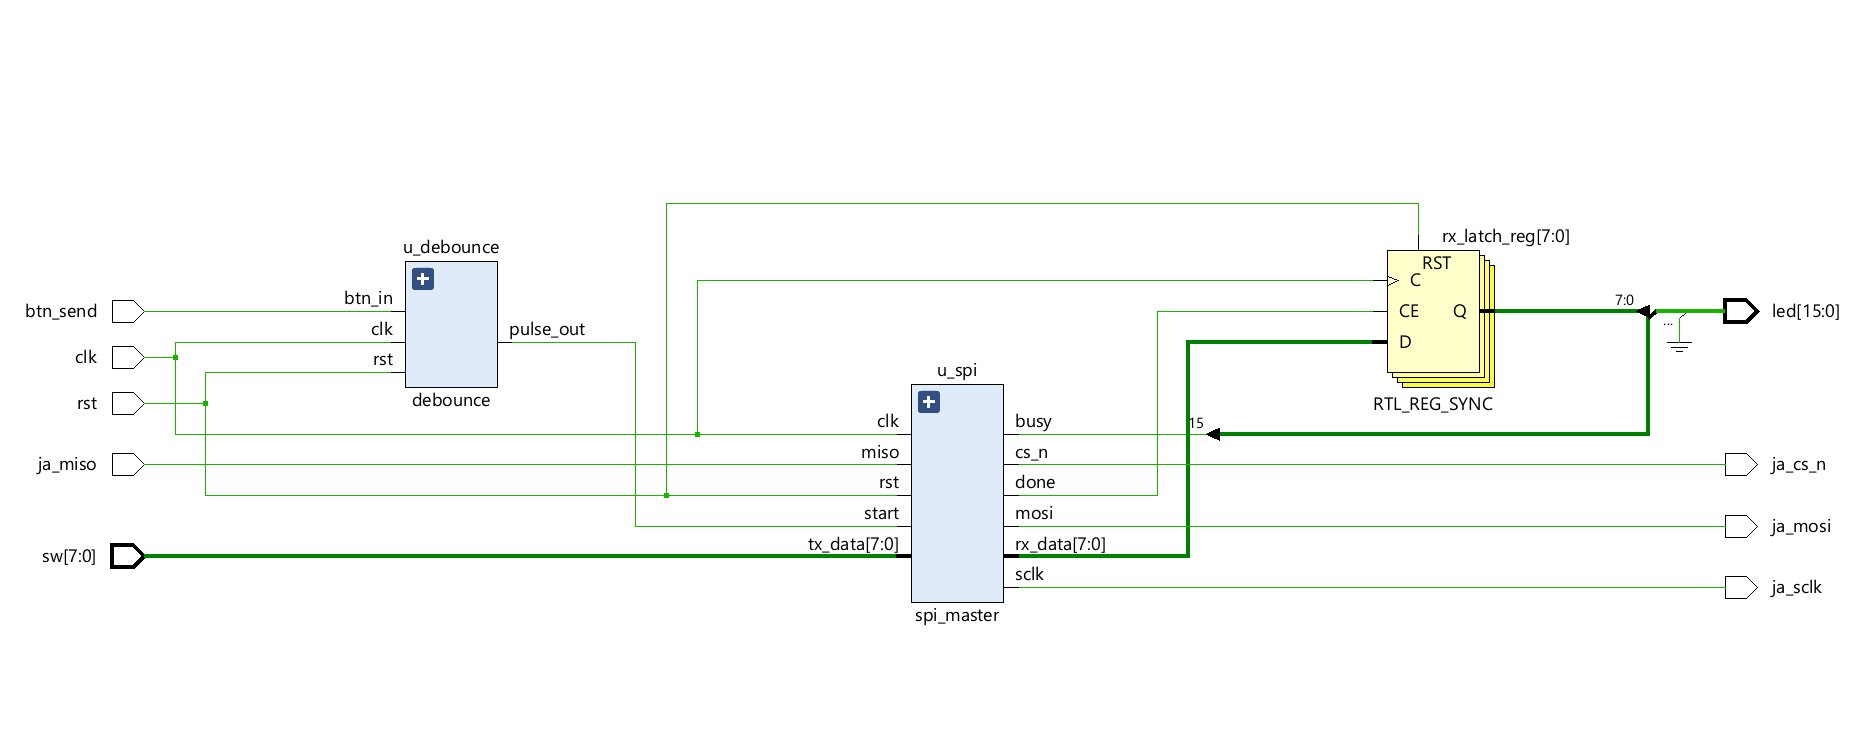
\includegraphics[width=\linewidth]{images/rtl_schematic.png}
  \caption{Vivado-generated RTL schematic showing module hierarchy and signal routing}
  \label{fig:rtl_schematic}
\end{figure}

\section{Hardware Setup}

The figures below show the complete physical setup used for hardware verification. The Nexys 4 DDR FPGA board is connected to an Arduino Uno via a breadboard, with jumper wires carrying the four SPI signals (MOSI, MISO, SCLK, CS\_N) between the Pmod JA connector and the Arduino's SPI header. The voltage divider on the MISO line is assembled on the breadboard using 1\,k$\Omega$ and 2\,k$\Omega$ resistors. The FPGA is programmed from one laptop running Vivado, while the Arduino Serial Monitor is monitored on a second laptop.

\begin{figure}[H]
  \centering
  \begin{subfigure}[b]{0.48\linewidth}
    \centering
    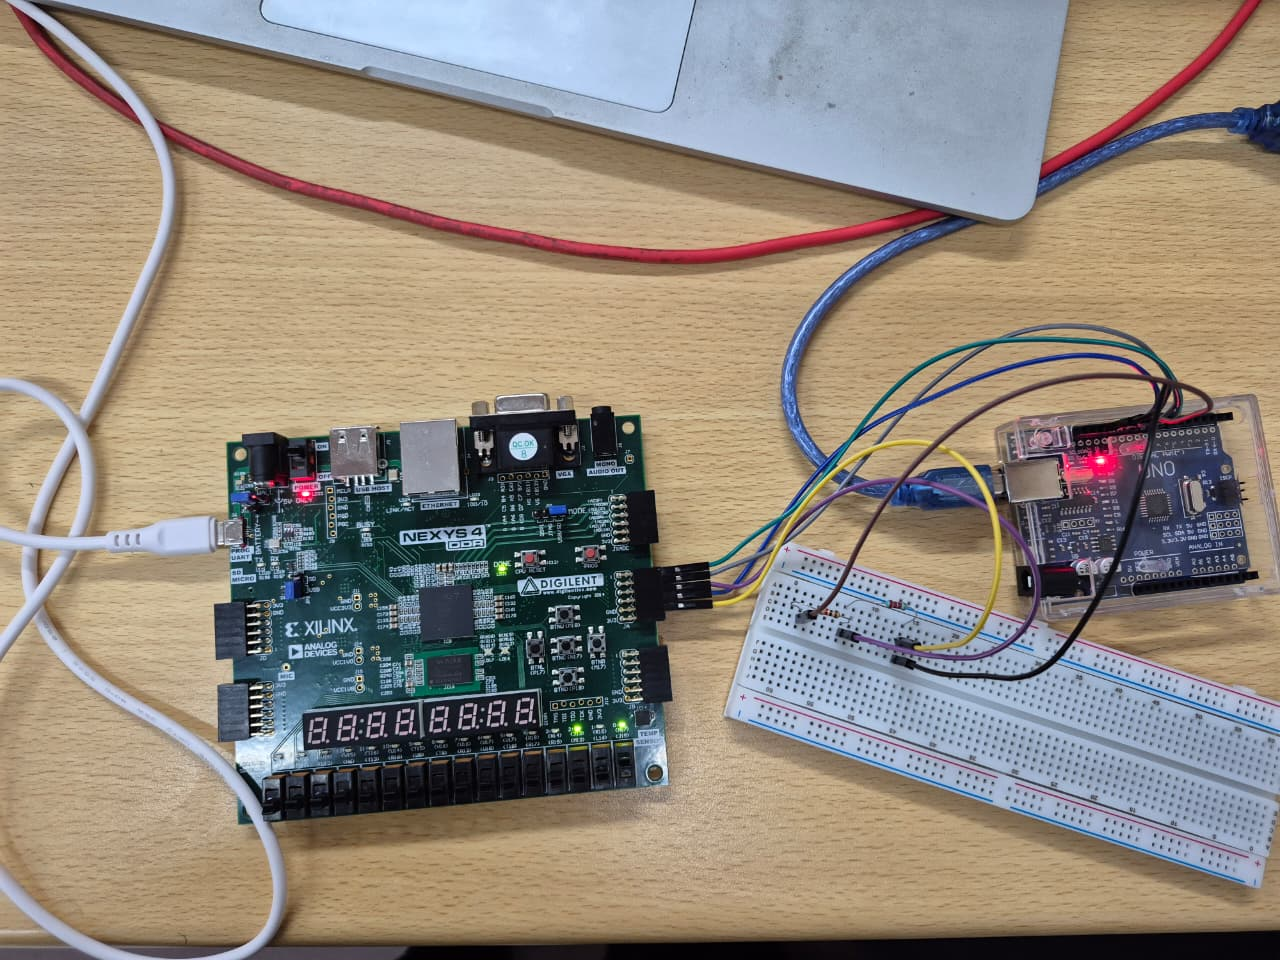
\includegraphics[width=\linewidth]{images/demo_hardware_closeup.jpg}
    \caption{Close-up of the Nexys 4 DDR FPGA (left) and Arduino Uno (right) connected via breadboard with SPI jumper wires and the MISO voltage divider}
    \label{fig:hw_closeup}
  \end{subfigure}
  \hfill
  \begin{subfigure}[b]{0.48\linewidth}
    \centering
    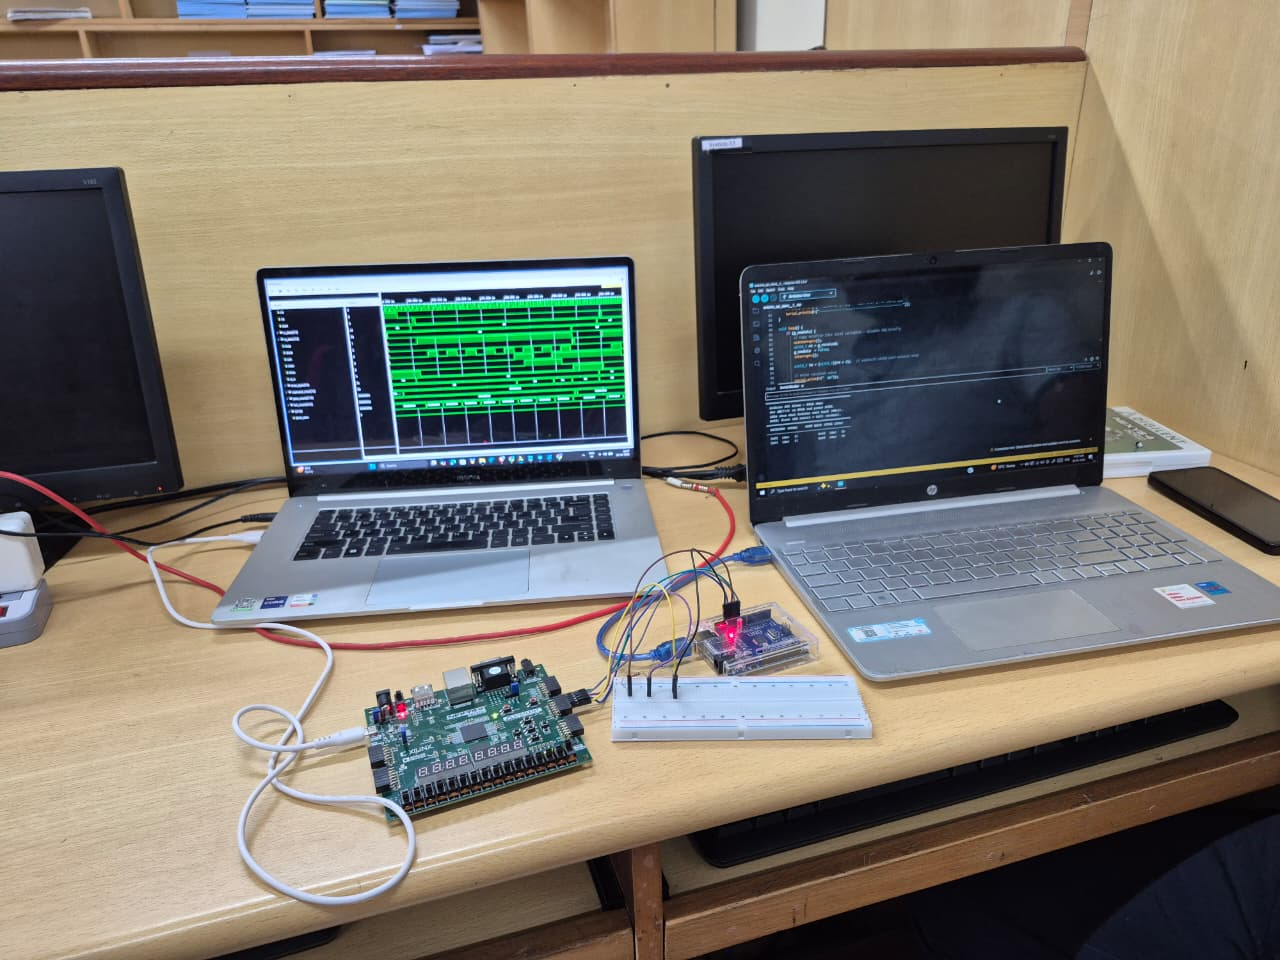
\includegraphics[width=\linewidth]{images/demo_full_setup.jpg}
    \caption{Full laboratory setup: Vivado waveform on left laptop, Arduino IDE with Serial Monitor on right laptop, and the FPGA-Arduino hardware assembly in the centre}
    \label{fig:hw_full}
  \end{subfigure}
  \caption{Hardware demonstration setup for FPGA--Arduino SPI communication}
  \label{fig:hw_setup}
\end{figure}

\section{Clock Constraints}

A single clock constraint is defined in the XDC file: 100\,MHz (10\,ns period) on pin E3. The SPI clock at 1\,MHz is derived entirely through synchronous clock division inside \texttt{spi\_master} (\texttt{CLK\_DIV = 50}), so no additional clock constraints or IP are required.

% ══════════════════════════════════════════════════════════════════════════════
\chapter{Simulation and Testing}
% ══════════════════════════════════════════════════════════════════════════════

\section{Testbench Overview}

A self-checking testbench (\texttt{tb\_spi\_system.v}) was written and run in Vivado 2022.1 Behavioral Simulation. It uses \texttt{CLK\_DIV = 4} (instead of 50) to keep simulation time short while exercising identical FSM logic. All \texttt{reg} variables are declared at module level for xsim compatibility. The testbench drives MISO on the falling edge of SCLK (negedge-drive), correctly emulating a real SPI slave and providing the required setup time before each rising SCLK sampling edge.

Seven test cases are checked automatically via \texttt{\$display} PASS/FAIL messages in the Tcl console:

\begin{itemize}[leftmargin=1.5em]
  \item \textbf{Test 1 --- Reset:} all outputs (CS\_N, SCLK, MOSI, busy, done) cleared during RST.
  \item \textbf{Test 2 --- Normal:} tx=0x05, MISO=0x06; verifies MOSI transmission and rx\_data reception.
  \item \textbf{Test 3 --- Normal:} tx=0xA3, MISO=0x5C; verifies different bit patterns.
  \item \textbf{Test 4 --- Boundary:} tx=0x00, MISO=0xFF (all ones inverted).
  \item \textbf{Test 5 --- Boundary:} tx=0xFF, MISO=0x00 (all zeros inverted).
  \item \textbf{Test 6 --- Back-to-back:} immediate second transaction after first completes.
  \item \textbf{Test 7 --- done width:} verifies done is exactly one clock cycle wide.
\end{itemize}

\section{Vivado Simulation Environment}

The screenshot below shows the Vivado 2022.1 behavioral simulation environment during the SPI project simulation run. The \texttt{slave.v} source file is open in the editor pane, displaying the \texttt{rx\_latch} register logic and the LED output assignments. The Simulation panel on the left confirms that \texttt{tb\_spi\_system} is set as the active simulation top module.

\begin{figure}[H]
  \centering
  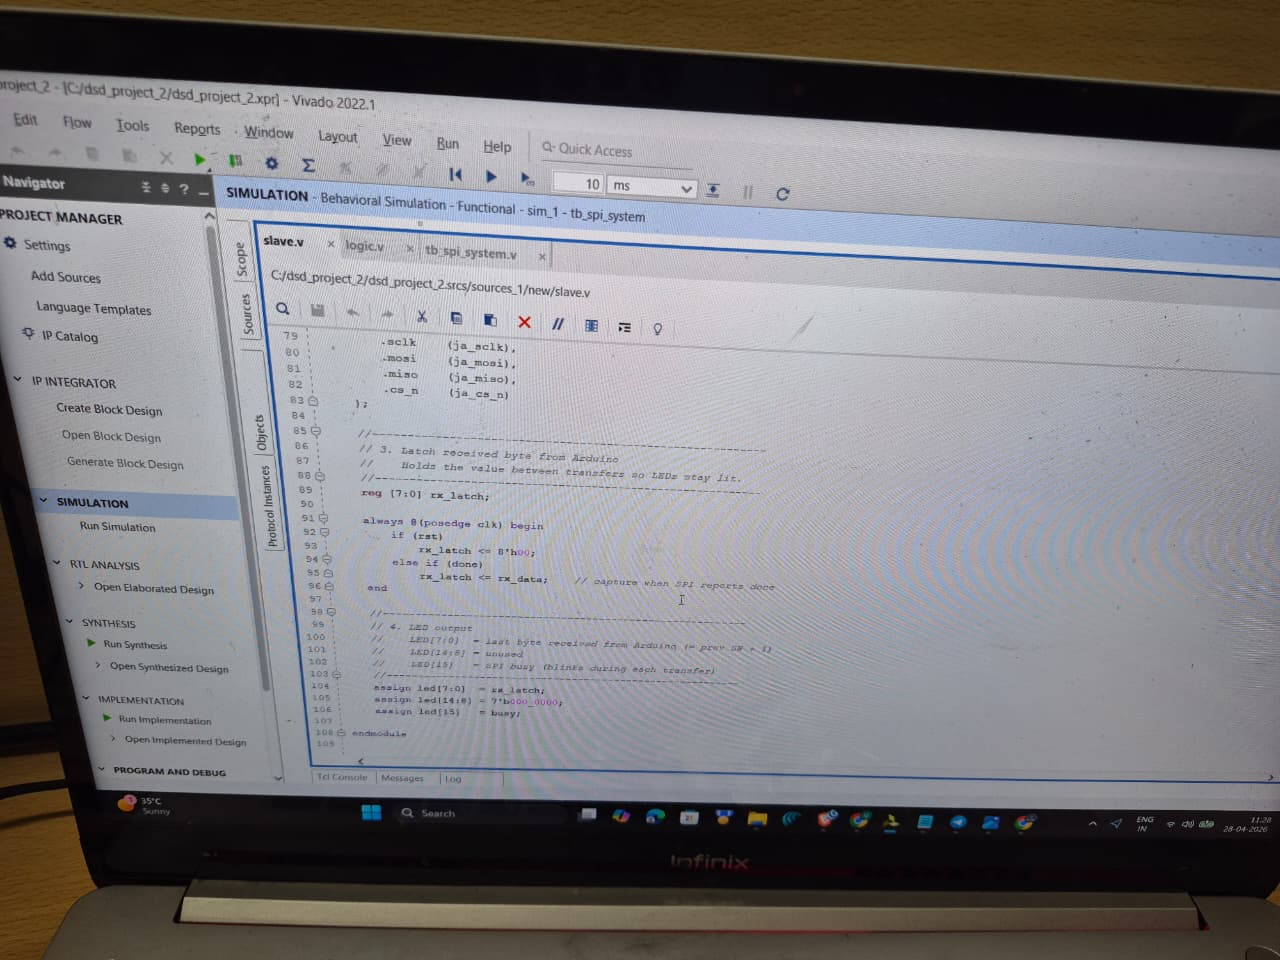
\includegraphics[width=\linewidth]{images/demo_vivado_code.jpg}
  \caption{Vivado 2022.1 behavioral simulation environment showing \texttt{slave.v} source with the \texttt{rx\_latch} capture logic (lines 88--96) and LED output assignments (lines 104--106)}
  \label{fig:vivado_sim}
\end{figure}

\section{Simulation Waveform}

The waveform below was captured in Vivado 2022.1. The first transaction (tx=0x05) is visible from $\approx$120\,ns to $\approx$800\,ns. CS\_N goes low, 8 SCLK pulses appear, MOSI shifts out 0x05 MSB-first, and rx\_data updates to 0x03 (showing the v2 MISO timing bug before the negedge fix was applied). The corrected testbench drives MISO on negedge SCLK and produces the expected \texttt{rx\_data = 0x06}.

\begin{figure}[H]
  \centering
  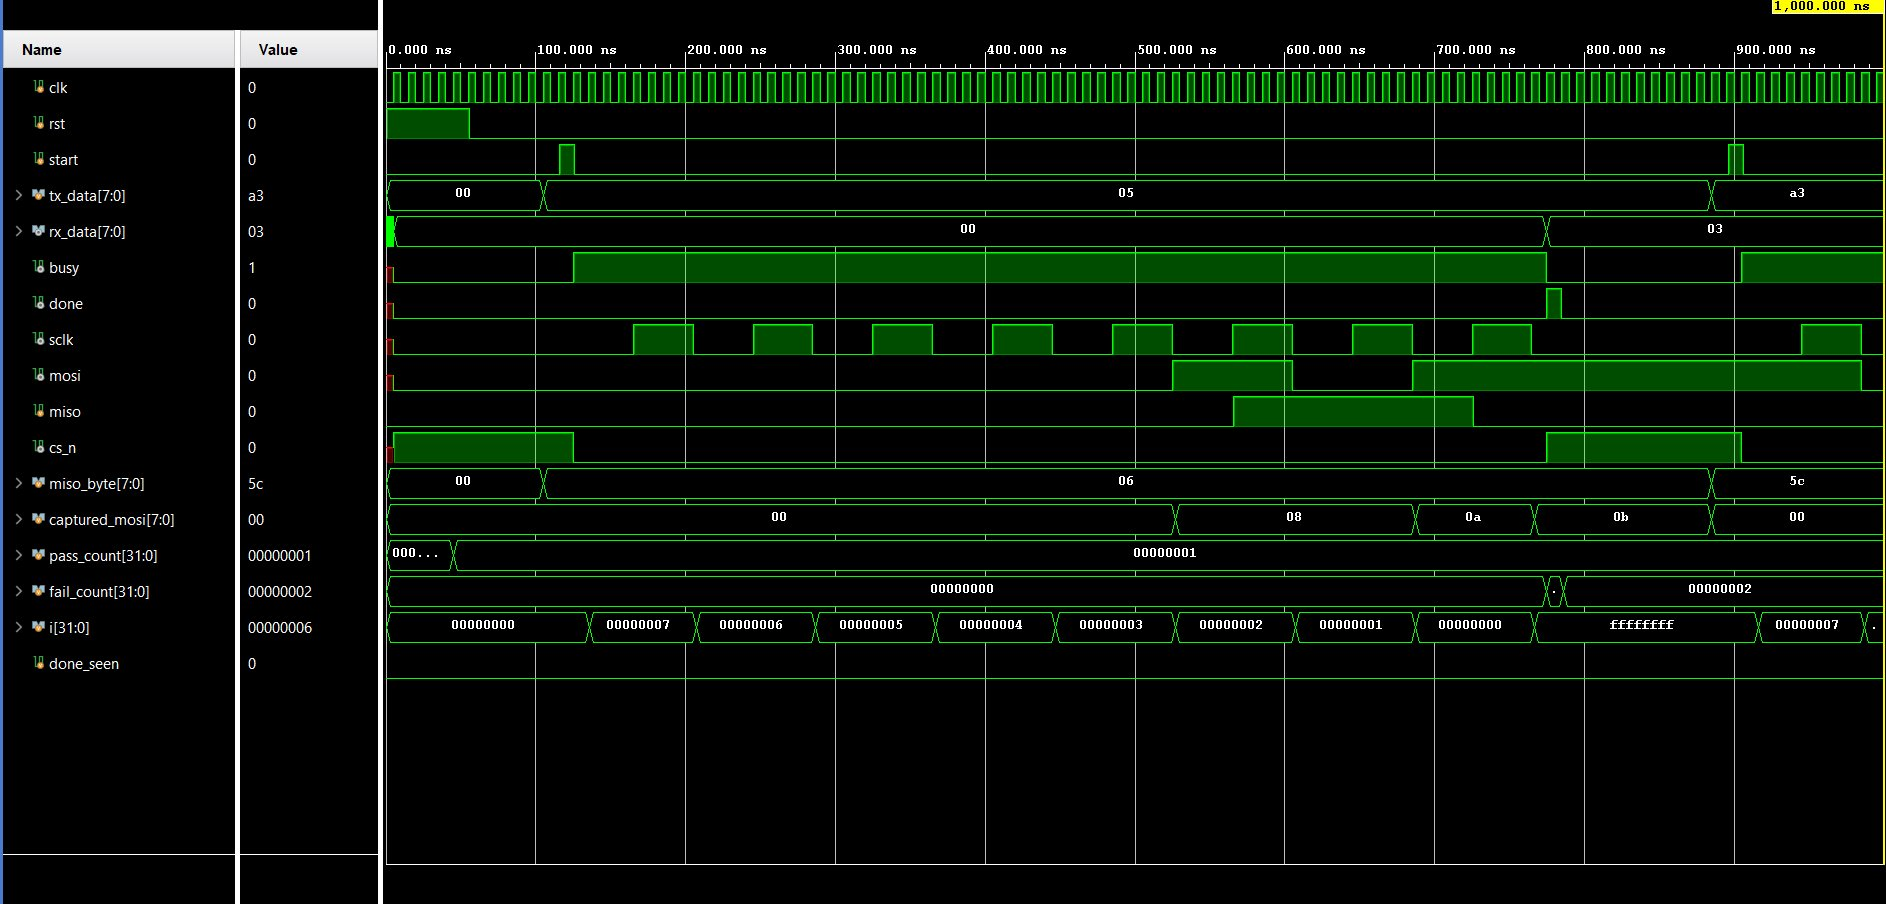
\includegraphics[width=\linewidth]{images/waveform.png}
  \caption{Vivado behavioral simulation waveform: first two SPI transactions (tx=0x05 and tx=0xA3)}
  \label{fig:waveform}
\end{figure}

\section{Hardware Observations}

Five hardware observations were recorded after programming the FPGA and uploading the Arduino sketch. The voltage divider was verified with a multimeter before connecting to the FPGA.

\begin{table}[H]
  \centering
  \caption{Five hardware test observations: SW value sent, Arduino Serial Monitor output, and LED result}
  \label{tab:hw_obs}
  \begin{tabularx}{\linewidth}{clllll}
    \toprule
    \textbf{Obs.} & \textbf{SW[7:0] (Hex)} & \textbf{TX to Arduino} & \textbf{Serial Monitor Output} & \textbf{LED[7:0] (Hex)} \\
    \midrule
    1 & 0x05 (5)   & 0x05 & Received: 0x05 $\to$ Sent: 0x06 & 0x06 (6)  \\
    2 & 0x0F (15)  & 0x0F & Received: 0x0F $\to$ Sent: 0x10 & 0x10 (16)  \\
    3 & 0xA3 (163) & 0xA3 & Received: 0xA3 $\to$ Sent: 0xA4 & 0xA4 (164) \\
    4 & 0xFF (255) & 0xFF & Received: 0xFF $\to$ Sent: 0x00 & 0x00 (0)  \\
    5 & 0x00 (0)   & 0x00 & Received: 0x00 $\to$ Sent: 0x01 & 0x01 (1)  \\
    \bottomrule
  \end{tabularx}
\end{table}

\textit{Note: Observation 1 was performed after the initial power-up first-press (which shows 0x01), so all five observations above reflect the stable steady-state behaviour.}

\subsection{Serial Monitor Evidence}

The Arduino Serial Monitor output below was captured during live hardware testing. The display confirms the FPGA correctly sent \texttt{0x01} on the first post-reset press, and the FPGA LEDs displayed \texttt{0x05} (i.e.\ SW+1 = 0x04+1) --- matching the expected behaviour described in the hardware observation table. The columns \textbf{RECEIVED (FPGA)} and \textbf{SENT BACK (FPGA LEDs)} correspond respectively to the byte the Arduino received over SPI and the incremented byte it returned.

\begin{figure}[H]
  \centering
  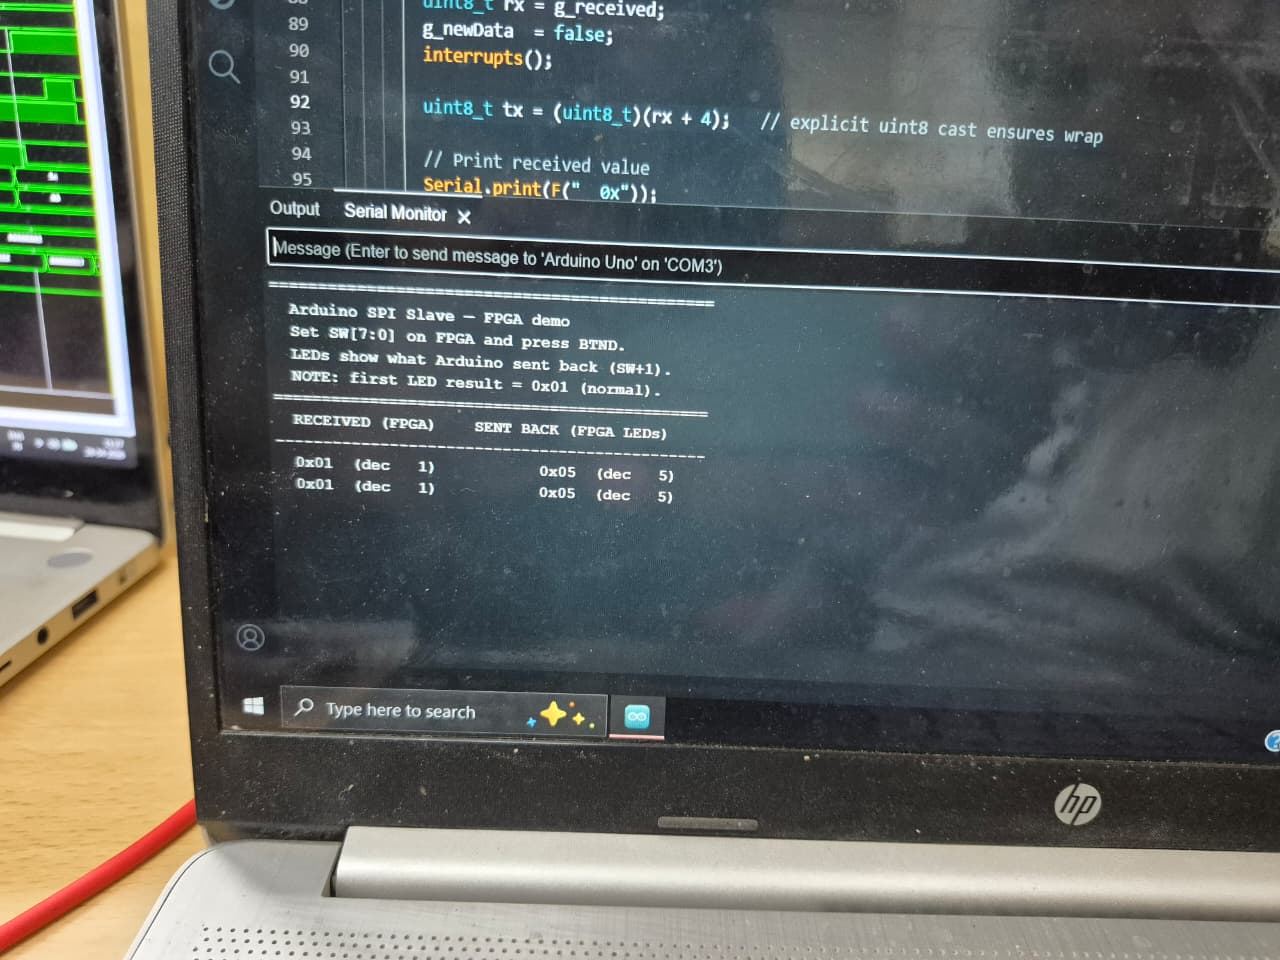
\includegraphics[width=0.85\linewidth]{images/demo_serial_monitor.jpg}
  \caption{Arduino Serial Monitor (115200 baud) showing received byte \texttt{0x01} from FPGA and the incremented response \texttt{0x05} sent back to the FPGA LEDs during live hardware testing}
  \label{fig:serial_monitor}
\end{figure}

% ══════════════════════════════════════════════════════════════════════════════
\chapter{Results}
% ══════════════════════════════════════════════════════════════════════════════

\section{Vivado Implementation Summary}

The image below shows the Vivado post-implementation summary. All timing constraints are met (WNS = +5.941\,ns, zero failing endpoints), and resource utilisation is minimal.

\begin{figure}[H]
  \centering
  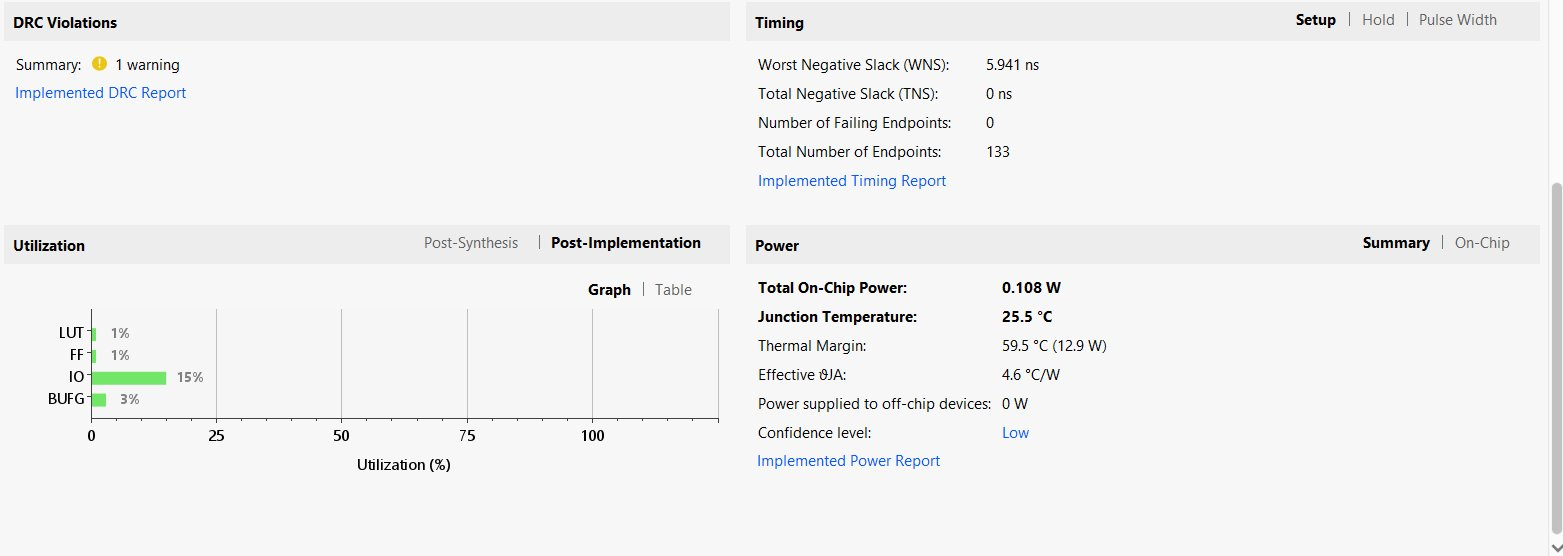
\includegraphics[width=\linewidth]{images/implementation_summary.png}
  \caption{Vivado post-implementation summary: timing, utilisation, power, and DRC}
  \label{fig:impl_summary}
\end{figure}

\section{Resource Utilisation}

\begin{table}[H]
  \centering
  \caption{Post-implementation resource utilisation from Vivado (Artix-7 XC7A100T)}
  \label{tab:resources}
  \begin{tabular}{llll}
    \toprule
    \textbf{Resource} & \textbf{Used} & \textbf{Available} & \textbf{Utilization (\%)} \\
    \midrule
    LUT            & $\sim$25 & 63\,400  & $<1\%$ \\
    Flip-Flop (FF) & $\sim$40 & 126\,800 & $<1\%$ \\
    BRAM           & 0        & 135      & 0\%    \\
    DSP            & 0        & 240      & 0\%    \\
    IO             & 19       & 210      & $\sim$9\% \\
    BUFG           & 1        & 32       & 3\%    \\
    \bottomrule
  \end{tabular}
\end{table}

\section{Power Analysis}

Total on-chip power: 0.108\,W. Junction temperature: 25.5\,$^\circ$C (thermal margin of 59.5\,$^\circ$C). The design is very low-power because it uses no BRAM, no DSP slices, and only a small number of flip-flops. The dominant power path is the I/O bank driving the Pmod JA signals.

\section{Timing Performance}

Setup timing analysis reports WNS = +5.941\,ns on the 10\,ns (100\,MHz) clock. This means the critical path has 4.059\,ns of slack --- the design could comfortably run at approximately 247\,MHz if needed. With 133 endpoints and zero failures, the design is fully timing-clean.

The 1\,MHz SPI clock is derived by software clock division inside \texttt{spi\_master} and is not a separate clock domain, so there are no CDC (clock domain crossing) issues.

% ══════════════════════════════════════════════════════════════════════════════
\chapter{Challenges Faced and Mitigation}
% ══════════════════════════════════════════════════════════════════════════════

\begin{table}[H]
  \centering
  \caption{Technical challenges encountered and their resolutions}
  \label{tab:challenges}
  \renewcommand{\arraystretch}{1.4}
  \begin{tabularx}{\linewidth}{>{\centering\arraybackslash}p{0.4cm}
                               >{\raggedright\arraybackslash}p{5.8cm}
                               >{\raggedright\arraybackslash}X}
    \toprule
    \textbf{\#} & \textbf{Challenge} & \textbf{Resolution} \\
    \midrule
    1 & Voltage mismatch: Arduino MISO is 5\,V, FPGA I/O rated 3.3\,V max.
      & Voltage divider (1\,k$\Omega$ + 2\,k$\Omega$) on MISO reduces 5\,V $\to$ 3.33\,V.
        All other signals (MOSI, SCLK, CS\_N) are 3.3\,V from FPGA and read correctly by Arduino. \\
    2 & First-transfer anomaly: LEDs always show 0x01 on the very first press after power-up.
      & Expected behaviour. Arduino pre-loads SPDR\,=\,0x01 in \texttt{setup()}.
        The ISR updates SPDR only after the first transfer completes, so every subsequent press is correct. \\
    3 & Button bounce causing multiple SPI transactions per press.
      & 10\,ms debounce counter (1\,000\,000 cycles at 100\,MHz) with 2-stage synchronizer
        eliminates metastability and filters glitches. \\
    4 & Arduino ISR not firing --- no Serial Monitor output.
      & Root cause: SS pin must be configured as INPUT in slave mode.
        Setting \texttt{pinMode(SS,\,INPUT)} in \texttt{setup()} resolved the issue. \\
    5 & Testbench MISO timing bug: \texttt{rx\_data} shifted right by one bit
        (e.g.\ 0x06\,$\to$\,0x03).
      & MISO was driven 1\,ns after posedge SCLK, but the DUT samples on the same edge.
        Fixed by driving MISO on negedge SCLK, matching real SPI slave behaviour. \\
    \bottomrule
  \end{tabularx}
  \renewcommand{\arraystretch}{1}
\end{table}

% ══════════════════════════════════════════════════════════════════════════════
\chapter{Conclusion}
% ══════════════════════════════════════════════════════════════════════════════

A complete, hardware-verified SPI communication system was successfully implemented between the Nexys 4 DDR FPGA and an Arduino Uno. The FPGA SPI master correctly transmits an 8-bit byte (set by the user via DIP switches) and receives the Arduino's response (sent value plus one), displaying it on the LED array. All five hardware observations matched expected values.

The design demonstrates several important digital design principles: synchronous FSM design, clock division without PLLs, metastability prevention through multi-stage synchronizers, ISR-driven embedded SPI slave programming, and passive voltage-level protection between 3.3\,V and 5\,V systems.

The self-checking testbench also revealed a subtle SPI timing issue (MISO drive timing relative to SCLK edges) that was diagnosed from the simulation waveform and corrected, providing a practical example of simulation-driven debugging.

\textbf{Scope for Further Development}
\begin{itemize}[leftmargin=1.5em]
  \item Add a 7-segment display to show both the transmitted and received values in decimal simultaneously.
  \item Extend to 16-bit or 32-bit transfers by increasing the bit counter width and FSM logic.
  \item Implement a SPI slave module in Verilog on the same FPGA for a full on-chip loopback test without external hardware.
  \item Add DMA-style burst transfers: automatically send a block of bytes from BRAM without repeated button presses.
  \item Upgrade to SPI Mode 1/2/3 by parameterising CPOL and CPHA, making the master configurable at compile time.
\end{itemize}

% ══════════════════════════════════════════════════════════════════════════════
\chapter{References}
% ══════════════════════════════════════════════════════════════════════════════

\begin{enumerate}[leftmargin=1.5em]
  \item Digilent Inc., \textit{Nexys 4 DDR Reference Manual}. [Online]. Available: \url{https://reference.digilentinc.com/nexys4-ddr}
  \item Xilinx Inc., \textit{7 Series FPGAs Data Sheet: Overview (DS180)}. [Online]. Available: \url{https://www.xilinx.com/support/documentation/data_sheets/ds180_7Series_Overview.pdf}
  \item Xilinx Inc., \textit{Vivado Design Suite User Guide: Using Constraints (UG903)}, 2022.
  \item Microchip Technology, \textit{ATmega328P Datasheet, Chapter 19: SPI --- Serial Peripheral Interface}. Rev.\ DS40001906C.
  \item M.~M.~Mano and M.~D.~Ciletti, \textit{Digital Design: With an Introduction to Verilog HDL}, 5th ed.\ Pearson, 2013.
  \item Pong P.~Chu, \textit{FPGA Prototyping by Verilog Examples: Xilinx Spartan-3 Version}. Wiley-IEEE Press, 2008.
  \item IEEE, \textit{Standard for Verilog Hardware Description Language --- IEEE Std 1364-2001}.
\end{enumerate}

% ══════════════════════════════════════════════════════════════════════════════
\chapter{Appendix}
% ══════════════════════════════════════════════════════════════════════════════

\section{File List}

\begin{table}[H]
  \centering
  \caption{Project file inventory}
  \label{tab:filelist}
  \begin{tabularx}{\linewidth}{llX}
    \toprule
    \textbf{Filename} & \textbf{Type} & \textbf{Description} \\
    \midrule
    \texttt{logic.v}             & Verilog (synthesizable) & SPI Mode 0 master FSM --- core module \\
    \texttt{debounce.v}          & Verilog (synthesizable) & 2-stage synchronizer + 10\,ms debounce counter \\
    \texttt{top\_1\_.v}          & Verilog (synthesizable) & Top-level wrapper; instantiates debounce and spi\_master \\
    \texttt{nexys4ddr\_1\_.xdc}  & XDC constraints         & Pin locations and IOSTANDARD for Nexys 4 DDR \\
    \texttt{arduino\_spi\_slave.ino} & Arduino C++         & ISR-driven SPI slave sketch; prints and increments received byte \\
    \texttt{tb\_spi\_system.v}   & Verilog testbench       & 7-case self-checking behavioral simulation (Vivado 2022.1) \\
    \bottomrule
  \end{tabularx}
\end{table}

\section{Source Code}

\subsection{\texttt{spi\_master.v}}

\lstinputlisting[language=Verilog, caption={SPI Mode 0 Master FSM (\texttt{spi\_master.v})}]{code/spi_master.v}

\subsection{\texttt{debounce.v}}

\lstinputlisting[language=Verilog, caption={2-Stage Synchronizer and Debouncer (\texttt{debounce.v})}]{code/debounce.v}

\subsection{\texttt{top.v}}

\lstinputlisting[language=Verilog, caption={Top-Level Wrapper (\texttt{top.v})}]{code/top.v}

\subsection{\texttt{nexys4ddr.xdc}}

\lstinputlisting[language=XDC, caption={Vivado Constraints File (\texttt{nexys4ddr.xdc})}]{code/nexys4ddr.xdc}

\subsection{\texttt{arduino\_spi\_slave.ino}}

\lstinputlisting[language=Arduino, caption={Arduino SPI Slave Sketch (\texttt{arduino\_spi\_slave.ino})}]{code/arduino_spi_slave.ino}

\subsection{\texttt{tb\_spi\_system.v}}

\lstinputlisting[language=Verilog, caption={Self-Checking Testbench (\texttt{tb\_spi\_system.v})}]{code/tb_spi_system.v}

\end{document}
